\section{Graph Coloring}

\subsection{Independent Sets and Bipartite Graphs}

\begin{definition}[Independent Set]
    Given a graph $G = (V,E)$, we say $A \subseteq V$ is \textit{\textbf{independent}} if and only if no no vertices in $A$ are adjacent.
\end{definition}

The only independent sets in $K_n$ are singletons. We can prove this using a contradiction and the definition of a complete graph and independent set.

\begin{definition}[Bipartite Graph]
    We say a graph $G = (V,E)$ is \textit{\textbf{bipartite}} if and only if we can partition $V$ into two \textbf{disjoint} \textbf{independent} sets.
\end{definition}

A bipartite graph $(V_1 \cup V_2, E)$ is a complete bipartite graph iff every $v_1 \in V_1$ is connected to every vertex in $V_2$ and vice versa. We denote a complete bipartite graph by $K_{|V_1|,|V_2|}$ ($K$ with a subscript denoting the size of the left and right partition, respectively).

\begin{theorem} \label{thm:odd-length-cycle-bipartite}
    A graph is bipartite if and only it does not contain a circuit of odd length.
\end{theorem}

\begin{proof}
    \hfill

    ($\implies$): Let $G=(V,E)$ be a bipartite graph. In particular, $V = A \cup B$ for some $A,B \subseteq V$ such that $A \cap B = \emptyset$ and for all $\{a,b\} \in E$, $a \in A$ and $b \in B$. Suppose, for contradiction, that $G$ contains an odd-length cycle $C = v_1 v_2 \ldots v_{n} v_1$ of length $n$. Without loss of generality, suppose that $v_i$ and $v_{i+1}$ alternates between $A$ and $B$. So, $v_1 \in A$, $v_2 \in B$, $v_3 \in A$, and so on. If the cycle is not in that particular order, we can reindex the vertices and still have the same cycle.

    Then, for $k \in \{1,2,3,\ldots,n\}$,
    $$
    v_k \in \begin{cases}
        A & \text{$k$ is odd} \\
        B & \text{$k$ is even}
    \end{cases}
    $$
    Since $C$ is a cycle of odd length, $n$ is odd. It follows that $v_n \in A$. But then, since $v_1 \in A$ and $\{v_n, v_1\} \in E$, this is a contradiction to the assumption that $G$ is bipartite.

    ($\impliedby$): Let $G=(V,E)$ be a graph. Without loss of generality, assume that $G$ is connected. Otherwise, we can consider the connected components individually. Assume that $G$ contains no odd cycle. Let $w \in V$ be a vertex in $G$.

    Let $A$ be the set of vertices whose shortest distance from $w$ is even, and let $B$ be the set of vertices whose shortest distance from $w$ is odd. That is,
    $$
    \begin{aligned}
        A = \{ v \in V \mid d(v,w) \equiv 0 \mod 2 \} \\
        B = \{ v \in V \mid d(v,w) \equiv 1 \mod 2 \}
    \end{aligned}
    $$
    Since $G$ is connected, every vertex is either at an even distance or odd distance from $w \in V$. A vertex cannot be both at an even distance and an odd distance from $w$ at the same time. Hence, $A \cup B = V$ and $A \cap B = \emptyset$. This implies that $A$ and $B$ are a valid partition of $V$.
    
    Now, we would like to show that $G$ is bipartite. It suffices to show for all vertices $a_1,a_2 \in V$ and $b_1,b_2 \in B$, $\{a_1,a_2\} \not\in E$ and $\{b_1,b_2\} \not\in E$. To prove this fact, we suppose the contrary and derive a contradiction. So, suppose that there does exist such $x,y \in A$ or $x,y \in B$ such that $\{x,y\} \in E$. Fix such $x,y$. We can assume that $x \neq y \neq w$. Otherwise, we have $w = x$ and $d(x,w) = 0$. Since $x$ and $y$ are in the same partition, $d(y,w)$ is even and $d(y,x) = 0$. However, this is not possible since $d(y,x) = 1$, which is odd. By a similar argument, we can show that $w \neq y$ either.
    
    To obtain a contradiction, we consider the shortest path from $x$ to $w$ and the shortest path from $y$ to $w$. Let $p$ be the shortest path from $x$ to $w$, and let $q$ be the shortest path from $y$ to $w$. Let $z$ be the last common vertex of $p$ and $q$. Note that $z$ may be $w$. We also note that $|p|$ and $|q|$ have the same parity since we assumed that $y,x$ are in the same partition.

    \begin{figure}[htbp]
        \centering
        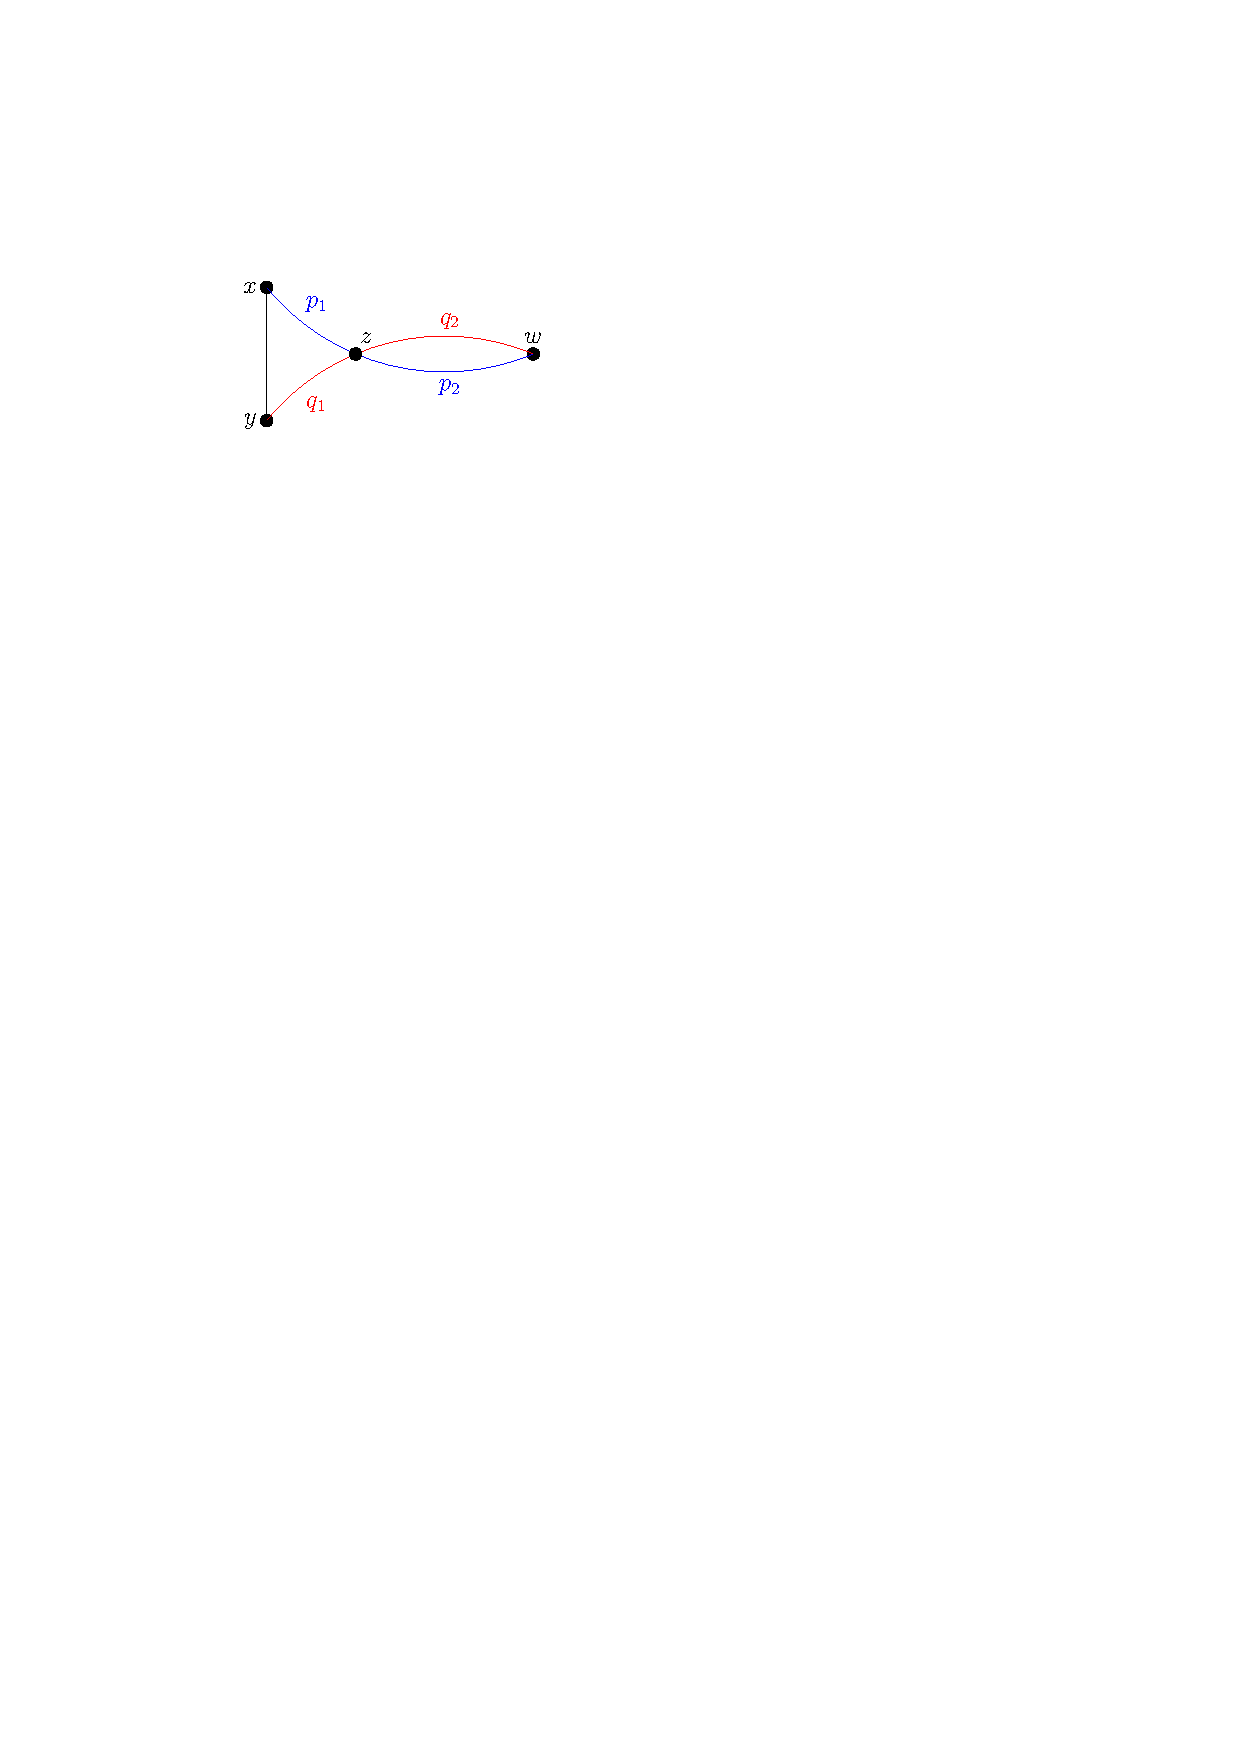
\includegraphics[width=0.3\linewidth]{figures/odd-length-cycle-bipartite.pdf}
        \caption{$p$ is the shortest path from $x$ to $w$. $q$ is the shortest path from $y$ to $w$. $p_1$ is the part of $p$ from $x$ to the last common vertex of $p$ and $q$. Similarly, $q_1$ is the part of $q$ from $y$ to the last common vertex of $p$ and $q$.}
        \label{fig:odd-length-cycle-bipartite}
    \end{figure}
    
    Let $p_1 = x \leadsto_p z$ be the part of the path $p$ from $x$ to $z$. Similarly, let $p_2 = z \leadsto_p w$, $q_1 = y \leadsto_q z$, and $q_2 = z \leadsto_q w$. We claim that $|p_2| = |q_2|$ since otherwise we can obtain a shorter path from $x$ to $w$ or from $y$ to $w$. Further, we claim that $|p_1|$ and $|q_1|$ have the same parity becuase $|p|$ and $|q|$ have the same parity and the second part of both paths, $p_2$ and $q_2$, are of the same length. Recall that $\{x,y\} \in E$. Then, $C = x \leadsto_{p_1} z \leadsto_{q_1} y \to x$. Since $|p_1|$ and $|q_1|$ have the parity, $|C| = |p_1| + |q_1| + 1$ is odd. This is becuase $|p_1| + |q_1|$ can be expressed as $2k$ for some $k \in \Z$. This is an odd-length cycle, which is a contradiction to our initial assumption that $G$ has no odd cycle. The only additional assumption leading to this contradiction is that $G$ is not bipartite. Hence, $G$ must be bipartite.
\end{proof}

\subsection{Coloring}

\begin{definition}[Proper Coloring]
    Let $G = (V,E)$ be a graph. A (proper) \textit{\textbf{coloring}} of $G$ is a function $\phi:\; V \to [k]$ such that for all $i \in [k]$, $\phi^{-1}(i)$ is independent. Equivalently, $\phi$ is a (proper) coloring of $G$ iff $\forall \{a,b\} \in E.\, \phi(a) \neq \phi(b)$. We call $\phi$ a $k$-coloring.
\end{definition}

\begin{definition}[Chromatic Number]
    The \textit{\textbf{chromatic number}} of a graph $G$, is the smallest $k$ such that there is a proper $k$ coloring of $G$. The chromatic number of $G$ is denoted by $\chi(G)$.
\end{definition}

\begin{theorem}
    A graph is 2-colorable if and only if it does not contain an odd-length cycle.
\end{theorem}

\begin{proof}
    Theorem \ref{thm:odd-length-cycle-bipartite} states that a graph is bipartite iff there is no odd-length cycle. To prove this theorem, it suffices to prove that a graph is 2-colorable if and only if the graph is bipartite.

    ($\implies$): Let $G = (V,E)$ be a 2-colorable graph. Take the coloring. Assign vertices with one color to $V_1$ and vertices with another color to $V_2$. $V_1$ and $V_2$ is a partition of $V$. By definition of a 2-color, for all $x,y \in V_1$, $\{x,y\} \not\in E$ and for all $x,y \in V_2$, $\{x,y\} \not\in E$.

    ($\impliedby$): Let $G=(V,E)$ be a bipartite graph where $V = V_1 \cup V_2$ is a partition. Assign one color to all vertices in $V_1$ and assign another color to all vertices in $V_2$. It is easy to prove that this is a valid 2-coloring directly from the definition of a bipartite graph.
\end{proof}

To demonstrate the concept of graph coloring and chromatic number, we consider the Petersen graph.

\begin{figure}[htbp]
    \centering
    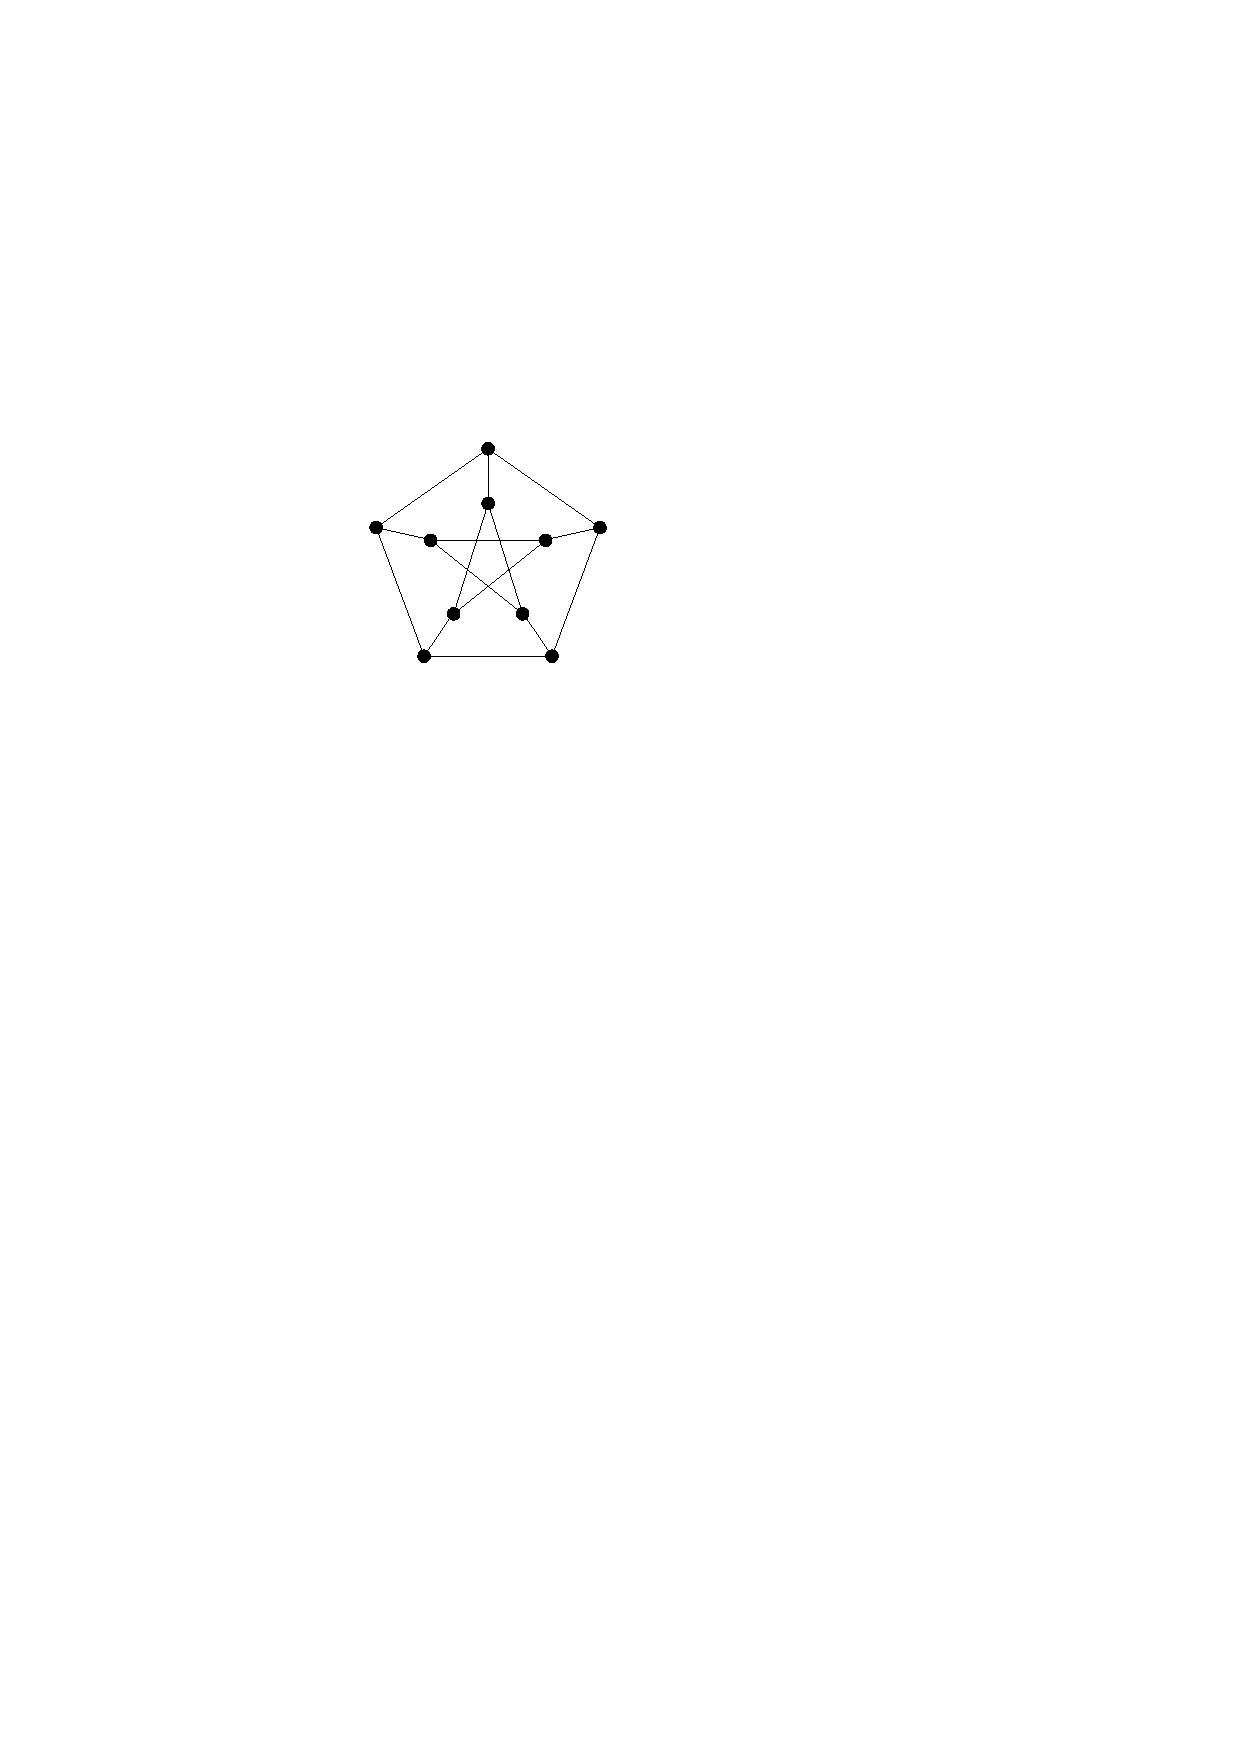
\includegraphics[width=0.2\linewidth]{figures/peterson-graph.pdf}
    \caption{The Petersen graph.}
    \label{fig:petersen-graph}
\end{figure}